\appendix
%%%%%%%%%%%%%%%%%%%%%%%%%%%%%%%%%%%%%%%%%%%%%%%%%%%%%%%%%%%%%%%%%%%%%%
\chapter[Analysis of Ghiya et. al.~\cite{Ghiya96}]{Analysis of Ghiya et. al.~\cite{Ghiya96}\footnote{The contents of this section are borrowed from ~\cite{Ghiya96}}}
%%%%%%%%%%%%%%%%%%%%%%%%%%%%%%%%%%%%%%%%%%%%%%%%%%%%%%%%%%%%%%%%%%%%%%
Most of the definitions and technical terms used in this chapter are borrowed from the aforementioned paper.
The proposed shape analysis composed of three store-less
abstractions that are computed together at each program point.
For each heap directed pointer they approximated the attribute
shape and for each pair of heap directed pointers they approximated the 
direction and interference relationships between them. These three abstractions 
are defined formally as follows:

\begin{definition}
Given any heap-directed pointer $p$, the shape attribute p.shape is Tree, 
if in the data structure accessible from p there is a unique (possibly empty) access path 
between any two nodes (heap objects) belonging to it. It is considered to be DAG (directed acyclic graph), 
if there can be more than one path between any two nodes in this data structure, 
but there is no path from a node to itself (i. e, it is acyclic). 
If the data structure contains a node having a path to itself, p.shape is considered to be Cycle.
Note that as lists are special case of tree data structures, their shape is also considered as Tree.
\end{definition}

\begin{definition}
Given two heap directed pointers $p$ and $q$, the direction matrix $D$ captures the following 
relationships between them:
\begin{itemize}
\item $D[p,q] = 1 : $ An access path possibly exists in the heap, from the heap object pointed to by $p$,
to the heap object pointed to by $q$. In this case we simply say that the pointer $p$ has a path to 
pointer $q$.
\item $D[p,q] = 0 : $ No access path exists from the heap object pointed to by $p$ to the heap object pointed to by $q$. 
\end{itemize}
\end{definition}

\begin{definition}
Given two heap directed pointers $p$ and $q$, the direction matrix $I$ captures the following 
relationships between them:
\begin{itemize}
\item $I[p,q] = 1 : $ A common heap object can be possibly accessed starting from pointers $p$ and $q$.
In this case we state that pointers $p$ and $q$ can interfere.
\item $I[p,q] = 0 : $ No common heap object can be accessed starting from pointers $p$ and $q$.
In this case we state that pointers $p$ and $q$ do not interfere.
\end{itemize}
\end{definition}

Direction relationships are used to actually estimate the shape attributes, where the interference 
relationships are used for safely calculating direction relationships. 

\subsection*{Illustrative Example}

The direction and interference matrices are illustrated in Fig.~\ref{fig:relwork_1}.
Part (a) represents a heap structures at a program point, while parts (b) and (c) show the direction 
and interference matrices for it.  
\begin{figure}
\centering
\begin{tabular}{c@{$\qquad\qquad$}c}
\multicolumn{2}{c}{
\scalebox{0.80} { 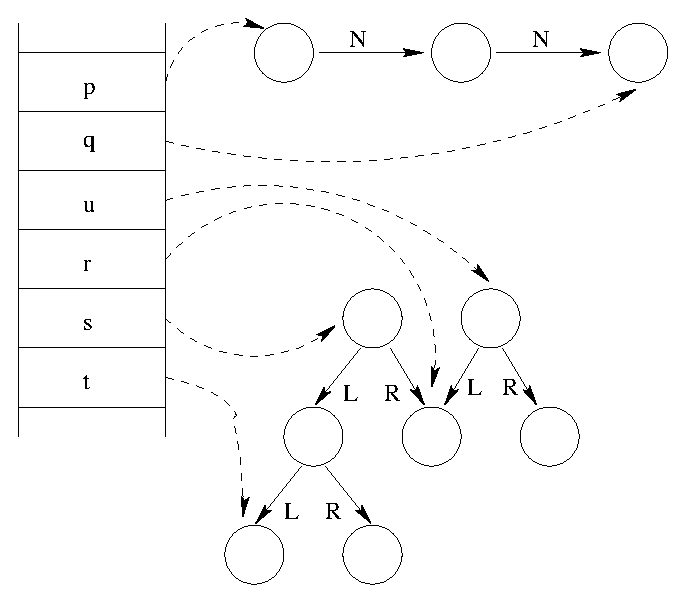
\includegraphics[scale=1]{diagrams/Appendix_2.eps}}
} \\
\multicolumn{2}{c}{
\scalebox{0.80}{ (a) Heap Structure }
} \\ \\
\scalebox{0.80} { \begin{tabular}{|c||c|c|c|c|c|c|}
\hline
$D$ & $p$ & $q$ & $r$ & $s$ & $t$ & $u$ \\ \hline \hline
$p$ & $1$ & $1$ & $0$ & $0$ & $0$ & $0$ \\ \hline 
$q$ & $0$ & $1$ & $0$ & $0$ & $0$ & $0$ \\ \hline 
$r$ & $0$ & $0$ & $1$ & $0$ & $0$ & $0$ \\ \hline 
$s$ & $0$ & $0$ & $1$ & $1$ & $1$ & $0$ \\ \hline 
$t$ & $0$ & $0$ & $0$ & $0$ & $1$ & $0$ \\ \hline 
$u$ & $0$ & $0$ & $1$ & $0$ & $0$ & $1$ \\ \hline 
\end{tabular}} 
& 
\scalebox{0.80} {\begin{tabular}{|c||c|c|c|c|c|c|}
\hline
$I$ & $p$ & $q$ & $r$ & $s$ & $t$ & $u$ \\ \hline \hline
$p$ & $1$ & $1$ & $0$ & $0$ & $0$ & $0$ \\ \hline 
$q$ & $1$ & $1$ & $0$ & $0$ & $0$ & $0$ \\ \hline 
$r$ & $0$ & $0$ & $1$ & $1$ & $0$ & $1$ \\ \hline 
$s$ & $0$ & $0$ & $1$ & $1$ & $1$ & $1$ \\ \hline 
$t$ & $0$ & $0$ & $0$ & $1$ & $1$ & $0$ \\ \hline 
$u$ & $0$ & $0$ & $1$ & $1$ & $0$ & $1$ \\ \hline 
\end{tabular}}  \\
\scalebox{0.80}{ (b) Direction Matrix}  & \scalebox{0.80} {(c) Interference Matrix}
\end{tabular}
\caption{Example Direction and Interference Matrices}
\label{fig:relwork_1}
\end{figure}


We now demonstrate how direction relationships help estimate the shape of the data structures.
In Fig.~\ref{fig:relwork_2}, initially we have both \p.\shape\ and \q.\shape\ as Tree. Further $D[q,p] == 1$, as there 
exists a path from \q\ to \p\ through {\tt next} link. The statement {\tt p$\rightarrow$prev = q}, sets up a path from
\p\ to \q\  through the {\tt prev} link. From direction matrix information we already know that a path exists
from \q\ to \p, and now a path is being set from \p\ to \q. Thus after the statement, $D[p,q] = 1$, $D[q,p] = 1$, \p.\shape\ = Cycle
and \q.\shape\ = Cycle.  

\begin{figure}
\centering
\scalebox{.80} {
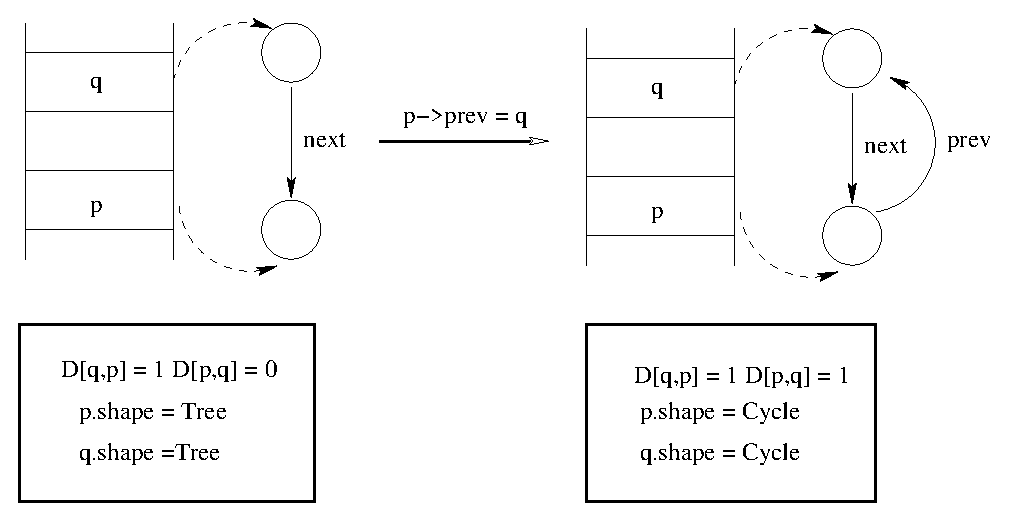
\includegraphics[scale=1]{Figure/figure_3}
}
\caption{Example Demonstrating Shape Estimation}
\label{fig:relwork_2}
\end{figure}

\subsection*{Analysis of Basic Statements}
They have considered eight basic statements that can access or
modify heap data structures as listed in Fig.~\ref{fig:relwork_3}(a). Variables \p\ and \q and the field $f$ are
of pointer type, variable $k$ is of integer type, and $op$ denotes the $+$ and $-$ operations. The 
overall structure of the analysis is shown in Fig.~\ref{fig:relwork_3}(b). Given the direction and the interference 
matrices $D$ and $I$ at a program point x, before the given statement, they compute the matrices $D_n$ and $I_n$
at a program point y. Additionally, we have the attribute matrix A, where for a pointer $p$, $A[p]$ gives its shape attribute.
The attribute matrix after the statement is presented as $A_n$.

For each statement they compute the set of direction and interference relationships it kills and generates. Using these sets, the
new matrices $D_n$ and $I_n$ are computed as shown in Fig.~\ref{fig:relwork_3}(c). Note that the elements in the gen and kill sets are denoted as $D[p,q]$
for direction relationships, and $I[p,q]$ for interference relationships. Thus a gen set of the form $\{D[x,y], D[y,z]\}$, indicates that
the corresponding entries in the output direction matrix $D_n[x,y]$ and $D_n[y,z]$ should be set to one. We also compute the set of 
pointers $H_s$, whose shape  attribute can be modified by the given statement. Another attribute matrix $A_c$ is used to store the 
changed attribute of pointers belonging to the set $H_s$. The attribute matrix $A_n$ is then computed using the 
matrices $A$ and $A_c$ as shown in Fig.~\ref{fig:relwork_3}(c).  

Let $H$ be the set of pointers whose relationships/attributes are abstracted by the matrices $D$. $I$ and $A$. Further
assume that updating an interference matrix entry $I[\q,\p]$, implies identically updating the entry $I[\p,\q]$.   
\begin{figure}
\centering
\scalebox{0.90}{
\begin{tabular}{|c|c|c|}
\hline
\begin{tabular}{l}
Allocation \\
1. {\tt p = malloc();} \\
\\
Pointer Assignments \\
2. {\tt p = q;} \\
3. {\tt p = \&(q$\rightarrow$f);} \\
4. {\tt p = q op k;} \\
5. {\tt p = NULL;} \\
6. {\tt p = q$\rightarrow$f;} \\
\\
Structure Updates \\
7. {\tt p$\rightarrow$f = q;} \\
8. {\tt p$\rightarrow$f = NULL;}
\end{tabular}  &
\begin{tabular}{c}
\scalebox{0.80}{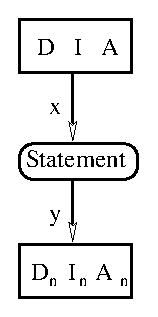
\includegraphics[scale=1]{diagrams/Appendix_4.eps}}
\end{tabular}
&
\begin{tabular}{l}
Build the new matrices\\
$\begin{array}{lll} 
\forall r,s \in H, & D_n[r,s] = D[r,s], & I_n[r,s] = I[r,s] \\
\forall s \in H, & A_n[s] = A[s]
\end{array}$ \\
\\
Delete Killed relationships \\
$\begin{array}{ll} 
\forall entries\ D[r,s] \in D\_kill\_set, & D_n[r,s] = 0\\  
\forall entries\ I[r,s] \in I\_kill\_set, & I_n[r,s] = 0\\  
\end{array}$ \\
\\
Add generated relationships \\
$\begin{array}{ll} 
\forall entries\ D[r,s] \in D\_gen\_set, & D_n[r,s] = 1\\  
\forall entries\ I[r,s] \in I\_gen\_set, & I_n[r,s] = 1\\  
\end{array}$ \\
\\
Update shape attributes of affected pointers \\
Compute $H_s$ and $A_s$ \\
$\begin{array}{ll} 
\forall s \in H_s, & A_n[s] = A[s]\\  
\end{array}$
\end{tabular}
\\
\scalebox{0.80}{(a) Basic statements} & \scalebox{0.80}{(b) Analysis Structure} & \scalebox{0.80}{(c) General Form of Analysis Rules} \\
\hline
\end{tabular}
}
\caption{The Overall Struture of the Analysis}
\label{fig:relwork_3} 
\end{figure}


The actual analysis rules can be divided into three groups: (1) allocations, (2) pointer assignments, and 
(3) structure updates. Figure~\ref{fig:relwork_4} shows the gen and kill sets corresponding to each statement. 
\begin{figure}[h]
\centering
\begin{tabular}{|l|c|}
\hline
1. {\tt p  = malloc();} &  
					$\begin{array}{lll}
						D\_kill\_set &=& \{D[p,s] \vert s \in H \wedge D[p,s]\}\ \cup\\
                                     &&   \{D[s,p] \vert s \in H \wedge D[s,p]\} \\
						I\_kill\_set &=& \{I[p,s] \vert s \in H \wedge I[p,s]\} \\
						D\_gen\_set &=& \{D[p,p]\} \quad I\_gen\_set = \{I[p,p]\} \\
						H_s &=& \{p\} \quad A_c[p] = Tree 	\\
					\end{array}$
								\\
\hline
\begin{tabular}{l}
2. {\tt p = q;} \\
3. {\tt p = \&(q$\rightarrow$f);} \\
4. {\tt p = q op k;} \\
\end{tabular}
 & 
				\begin{tabular}{l}
					Kill set same as that of {\tt p  = malloc();} \\
					$\begin{array}{lll}
						D\_gen\_set\_from &=& \{D[s,p] \vert s \in H \wedge s \not= p \wedge D[s,q]\} \\
						D\_gen\_set\_to &=& \{D[p,s] \vert s \in H \wedge s \not= p \wedge D[q,s]\} \\
						I\_gen\_set	&=& \{I[p,s] \vert s \in H \wedge s \not= p \wedge I[q,s]\}\ \cup \\
											&&  \{I[p,p] \vert I[q,q]\} \\
						D\_gen\_set	&=& D\_gen\_set\_from\ \cup D\_gen\_set\_to \\
						H_s &=& \{p\} \quad A_c[p] = A[q] 	\\
					\end{array}$
				\end{tabular}
								\\
\hline
5. {\tt p = NULL;} & 
				\begin{tabular}{l}
					Kill set same as that of {\tt p  = malloc();} \\
					$\begin{array}{lll}
						D\_gen\_set &=& \{\} \quad I\_gen\_set = \{\} \\
						H_s &=& \{p\} \quad A_c[p] = Tree 	\\
					\end{array}$
				\end{tabular}
								\\
\hline
6. {\tt p = q$\rightarrow$f;} & 
				\begin{tabular}{l}
					Kill set same as that of {\tt p  = malloc();} \\
					$\begin{array}{lll}
						D\_gen\_set\_from 	&=& \{D[s,p] \vert s \in H \wedge s \not= p \wedge I[s,q]\} \\
						D\_gen\_set\_to 	&=& \{D[p,s] \vert s \in H \wedge s \not= p \wedge s \not= q\ \wedge \\
                                            &&    D[q,s]\}\ \cup \{D[p,q] \vert A[q] = Cycle\}\ \cup \\
											&& \{D[p,p] \vert D[q,q]\} \\
						D\_gen\_set 		&=& D\_gen\_set\_from\ \cup D\_gen\_set\_to \\
						I\_gen\_set 		&=& \{I[p,s] \vert s \in H \wedge s \not= p \wedge I[q,s]\}\ \cup \\
											&&  \{I[p,p] \vert I[q,q]\} \\
						A_c[p] &=& A[q] 	\\
					\end{array}$
				\end{tabular}
								\\
\hline
7. {\tt p$\rightarrow$f = NULL;} & 
					$\begin{array}{lll}
						D\_kill\_set &=& \{\} \quad I\_kill\_set = \{\}\\
						D\_gen\_set 		&=& \{\} \quad I\_gen\_set  = \{\}\\
						A_c[p] &=& A[p]\ \forall p \in H  	\\
					\end{array}$
								\\
\hline
7. {\tt p$\rightarrow$f = q;} & 
				\begin{tabular}{l}
					Kill set same as that of {\tt p$\rightarrow$f = NULL;} \\
					$\begin{array}{lll}
						D\_gen\_set		&=& \{D[r,s] \vert r,s \in H \wedge D[r,p] \wedge D[q,s]\}  \\
						I\_gen\_set  	&=& \{I[r,s] \vert r,s \in H \wedge D[r,p] \wedge I[q,s]\} \\
					\end{array}$ \\ \\
					\underline{Pointer q already has a path to p, D[q,p] = 1} \\
					$\begin{array}{lll}
						H_s 			&=& \{s \vert s \in H \wedge (D[s,p] \vee D[s,q])\} \\
						D[q,p] &\Rightarrow& A_c[s] = Cycle\ \forall s \in H_s  	\\
					\end{array}$ \\ \\
					\underline{A[q] = Tree} \\
					$\begin{array}{lll}
						H_s 			&=& \{s \vert s \in H \wedge (D[s,p] \vee I[s,q])\} \\
						(\neg D[q,p] \wedge (A[q] = Tree)) &\Rightarrow& A_c[s] = A[s] \Join Dag\ \forall s \in H_s  	\\
					\end{array}$ \\ \\
					\underline{A[q] $\not=$ Tree} \\
					$\begin{array}{lll}
						H_s 			&=& \{s \vert s \in H \wedge D[s,p]\} \\
						(\neg D[q,p] \wedge (A[q] \not= Tree)) &\Rightarrow& A_c[s] = A[s] \Join A[q]\ \forall s \in H_s  	\\
					\end{array}$
				\end{tabular}
								\\
\hline							
\end{tabular}
\caption{Analysis Rules}
\label{fig:relwork_4}
\end{figure}


%%%%%%%%%%%%%%%%%%%%%%%%%%%%%%%%%%%%%%%%%%%%%%%%%%%%%%%%%%%%%%%%%%%%%%
\chapter[Analysis of Marron et. al.~\cite{marron06static}]{Analysis of Marron et. al.~\cite{marron06static}\footnote{The contents of this section are borrowed from ~\cite{marron06static}}}
%%%%%%%%%%%%%%%%%%%%%%%%%%%%%%%%%%%%%%%%%%%%%%%%%%%%%%%%%%%%%%%%%%%%%%
Most of the technical terms used in this chapter are borrowed from the aforementioned paper.
The proposed analysis followed the abstract heap graph model that uses nodes to
represent sets of concrete cells (heap allocated objects and arrays) and edges to represent sets of pointers. 
Each node in the abstract heap graph can be viewed as a region in memory on which certain
layout predicates can be defined (Tree Layout, List Layout, Singleton Layout, Multi-Path or Cycle Layouts)
which signifies what types traversal patterns a program can use to navigate through the data
structures in the region. To track the concrete Structure Layout, they introduce a simple domain of 
layout types = \{Singleton, List, Tree, Multi-Path, Cycle\}. The abstract layouts can be given a simple
total order: Singleton < List < Tree < Multi-Path < Cycle. This order can be interpreted as: if
a node n has abstract layout $\zeta$ then the concrete region, $\mathcal{R} = \gamma(n)$, where $\gamma$ is the concreatization
operator, may have any of the layout properties less than or equal to $\zeta$. For example, if we have a node
with layout type List the concrete region may have the List or Singleton layout properties. If the
node has Cycle as the layout then the concrete domain may have any of the layout properties. The
abstract layout for a node n represents the most general concrete layout that may be encountered
by a program traversing the region that is represented by the node n.

In their analysis, sometimes refinement is necessary (after summarization the abstract heap graph) whose 
purpose is to transform summary representations into forms that make certain relationships explicit, so that the information
 in these relationships can be utilized more easily. During refinement they turn summary nodes 
into a number of nodes of size one so that strong updates can be performed and exact relations 
between variables can be maintained. 

In order to eliminate the state explosion that is possible with refinement, they adopt the approach
of only doing refinement in those cases in which we can be sure that there is a unique way in which
new nodes can be materialized. This limits the level of details that can be achieved, but it 
is easy to demonstrate scenarios where refinement into multiple possibilities is needed to get results with the
desired accuracy. 
